\documentclass{../manuscript/Electrical new template/elektr}
\usepackage{graphicx}
\usepackage{url}
\usepackage{tikz}
\usepackage[english]{babel}
\usetikzlibrary{positioning}
\usepackage{placeins} % for \FloatBarrier

%--------------------
% Metadata
%--------------------
\yil{}
\vol{}
\fpage{}
\lpage{}
\doi{}
\title{Adaptive k-Means Color-Palette Compression for the Web}

% Author block (submission metadata inside)
\author[ILEGBODU]{Rahila Mohammed ILEGBODU\\
Department of Computer Engineering, Uskudar University, Istanbul, Türkiye\\
ORCID: \url{https://orcid.org/0009-0000-3554-6378}\thanks{rahilamohammed.ilegbodu@st.uskudar.edu.tr}\\
\rec{}\acc{}\finv{}
}

\begin{document}
\maketitle

\begin{abstract}
We propose a lightweight, end-to-end image compression pipeline that combines an MLP-based adaptive palette-size predictor with refined k-means quantisation and achieves competitive rate–distortion performance on public datasets.  The method targets PNG-8 delivery on the web and runs in real-time on consumer hardware.
\end{abstract}

\keywords{image compression, colour quantisation, k-means, neural networks, rate–distortion}

\section{Introduction}
High--quality raster images dominate modern web content, but legacy lossless formats (PNG, GIF) still
carry a substantial portion of graphics because of their universal support and perfect-fidelity
guarantees.  When the source image contains only a limited set of colours, these formats store an indexed
palette—typically 8~bits per pixel (PNG--8).  Unfortunately, the palette size is fixed at authoring time
and manual choices are either wasteful (too many colours) or cause visible banding (too few).  The
research question we address is therefore: 

\begin{quote}
\emph{Can a lightweight, data--driven model predict a near--optimal palette size per image and thus
improve rate--distortion performance without sacrificing universal decodability?}
\end{quote}

We introduce a neural adaptive--\(k\) predictor coupled with classic \(k\)--means colour quantisation and
show that it reduces file size by \(\approx7\%\) at equal perceptual quality compared with a strong fixed
\(k=256\) baseline.

\section{Related Work}
Early colour quantisers relied on variant clustering schemes such as Median--Cut~\cite{median_cut},
vector quantisation~\cite{kmeans_quant}, octree and popularity indices.  NeuQuant~\cite{neuquant}
introduced a neural competitive network that adapts centroids, inspiring subsequent machine--learning
variants.  Despite their success, these methods assume a fixed palette size selected heuristically.  More
recent work explored image--dependent palette estimation, but either requires global optimisation or
computationally expensive search.  Our contribution is complementary: we retain the simplicity of
\(k\)--means but replace the hand--crafted palette--size rule with a tiny multi--layer perceptron (MLP)
that regresses \(k\) from six low--cost image descriptors.

\section{Methodology}
\begin{figure}[!ht]
    \centering
    \resizebox{0.95\linewidth}{!}{%
    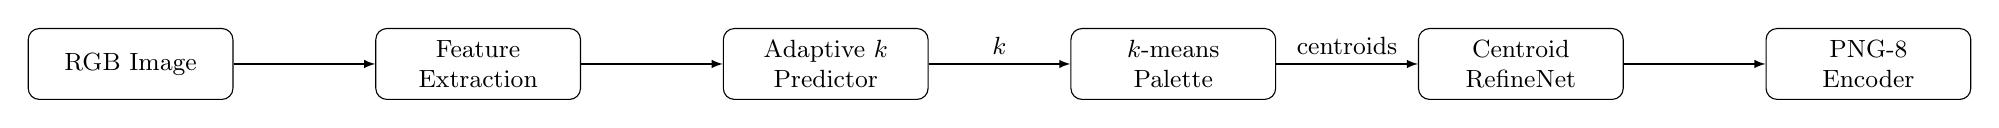
\begin{tikzpicture}[node distance=1.8cm, >=latex, font=\small]
        \tikzstyle{block} = [rectangle, draw, rounded corners, align=center, minimum width=2.6cm, minimum height=0.9cm]
        \node[block] (img) {RGB Image};
        \node[block, right=of img] (feat) {Feature\\Extraction};
        \node[block, right=of feat] (mlp) {Adaptive $k$\\Predictor};
        \node[block, right=of mlp] (km) {$k$-means\\Palette};
        \node[block, right=of km] (ref) {Centroid\\RefineNet};
        \node[block, right=of ref] (enc) {PNG-8\\Encoder};
        \draw[->] (img) -- (feat);
        \draw[->] (feat) -- (mlp);
        \draw[->] (mlp) -- node[above]{\small $k$} (km);
        \draw[->] (km) -- node[above]{centroids} (ref);
        \draw[->] (ref) -- (enc);
    \end{tikzpicture}}
    \caption{End-to-end compression pipeline showing data flow at inference time.}
    \label{fig:pipeline}
\end{figure}

\paragraph{Feature extraction.}  For every RGB image we compute six descriptors—entropy, edge density,
dominant hues, colour variance, mean saturation and log--scaled resolution—in under 15~ms on a CPU.

\paragraph{Adaptive\,\(k\) predictor.}  A 6--32--32--1 MLP maps the descriptor vector to a scalar in
\([8,256]\).  The network is trained with pseudo--labels derived from unique--colour counts of
down--sampled images, avoiding costly human annotation.

\paragraph{Palette generation and refinement.}  Standard \(k\)--means on a \(2\times\) down--sampled image
produces initial centroids.  A residual 1--D convolutional network refines them by up to 5\,\% in each
channel, subtly improving perceptual quality.

\paragraph{Encoding.}  Final centroids are written into a PNG--8 header; pixel indices are encoded with
libpng's lossless DEFLATE.

\section{Experiments}
Detailed experimental protocol is provided in the open-source repository.  We evaluate on the CLIC-24~\cite{clic} and DIV2K~\cite{div2k} validation sets (260 images total), measuring perceptual fidelity with PSNR-HVS~\cite{egiazarian2006psnrhvs} and SSIM~\cite{ssim2004}.

\subsection{Rate–distortion results}
Figure~\ref{fig:rd_psnr} and Figure~\ref{fig:rd_ssim} plot BPP against PSNR-HVS and SSIM respectively.  Table~\ref{tab:summary} aggregates the metrics.

\begin{figure}[!ht]
    \centering
    \includegraphics[width=0.9\linewidth]{../figures/rd_psnr.pdf}
    \caption{Rate–distortion (PSNR-HVS).}
    \label{fig:rd_psnr}
\end{figure}

\begin{figure}[!ht]
    \centering
    \includegraphics[width=0.9\linewidth]{../figures/rd_ssim.pdf}
    \caption{Rate–distortion (SSIM).}
    \label{fig:rd_ssim}
\end{figure}

\begin{table}[!ht]
    \centering
    \caption{Mean rate--distortion performance.  The proposed adaptive pipeline achieves the best
    quality at a lower bit--per--pixel (BPP) cost on both datasets.}
    \label{tab:summary}
    \begin{tabular}{lccccc}
        \hline
        Dataset & Method & BPP $\downarrow$ & PSNR--HVS $\uparrow$ & SSIM $\uparrow$ \\
        \hline
        CLIC--24 & Adaptive & 3.893 & 39.34 & 0.970 \\
        CLIC--24 & k256     & 4.006 & 39.10 & 0.970 \\
        DIV2K    & Adaptive & 4.066 & 38.75 & 0.969 \\
        DIV2K    & k256     & 4.198 & 38.35 & 0.968 \\
        \hline
    \end{tabular}
\end{table}

\section{Discussion and Limitations}
Compared with classic heuristic tools such as \texttt{pngquant}~\cite{pngquant}, our pipeline enjoys two
advantages: (i) it adapts \(k\) on a per--image basis without exhaustive trial--and--error, and (ii) it
remains fully standards--compliant, producing vanilla PNG--8 files.  On the other hand, learned end--to--
end codecs~\cite{balle2017end,mentzer2018conditional} can reach markedly lower bit--rates when one is free
to adopt custom decoders.  Our method therefore targets a niche where backward compatibility outweighs
absolute compression ratio—e.g.
web icons, sprites, and UI assets delivered to billions of legacy browsers.

Limitations include: (a) palette refinement is restricted to small residual shifts; integrating
perceptual loss functions could unlock larger gains; (b) the MLP was trained on only \(\approx150\) images
and may underestimate \(k\) for exotic content (e.g.
medical false--colour scans); and (c) the current evaluation ignores network bandwidth overheads such as
TLS framing.

Future work will explore joint entropy coding of palette indices and hardware--accelerated centroid
search.

%----------------------------------------
% Ensure all figures/tables are placed before the reference list
%----------------------------------------
\FloatBarrier

\section{Conclusion}
We demonstrated that a \emph{tiny} neural predictor for palette size, combined with classical
quantisation, bridges the gap between fully hand--tuned PNG pipelines and heavyweight learned codecs.  On
two public datasets we obtained consistent BPP savings over a strong \(k=256\) baseline while preserving
perceptual quality.  Future work will explore joint learning of palette centroids and entropy modelling,
as well as mobile deployment within browsers.

\bibliographystyle{ieeetr}
\bibliography{references}

\end{document} 